\chapter{Representational Geometry and Alignment in Neural Nets}
\label{ch:02-representational-geometry}

\lecturemeta{Phillip Isola}{MIT}

Isola's argument is that a representation should be identified with the distances it induces,
not with the coordinates it happens to use, and that almost everything interesting follows
from taking that seriously. If two networks encode the same distances in different bases they
are the same representation for practical purposes, so the right way to compare them is to
compare kernels. Once comparison is on that footing an empirical claim becomes measurable:
strong models trained on different data and different modalities are converging on one
kernel, and human perceptual judgements sit close to it. The lecture ends by turning this
from an observation into an engineering target, with the costs of doing so stated honestly.

\section*{Key ideas}

\paragraph{Every layer is a representation, and a representation is a point cloud.} A
representation is a map $\rep : \dom \to \mathcal{Z}$, usually with $\mathcal{Z} = \Rd$, and
the representation of a dataset is the set $Z = \{\rep(\xin^{(i)})\}_{i=1}^{n}$, a point
cloud in $\Rd$. Deep nets transform that cloud layer by layer, so the input data and the
output beliefs are representations too, not just the penultimate activations. The framing
pays off immediately in what a classifier is doing: deforming an input point cloud until the
classes land on the vertices of a simplex. The opening example is older, that object
detectors emerge in scene CNNs trained only on scene labels~\citep{zhou2015}, which
establishes that internal activations carry semantics nobody put there on purpose.

\paragraph{Comparing two clouds means choosing an invariance.} Representational similarity is
a function $d : \rep_1 \times \rep_2 \to \R$, in practice evaluated on finite samples $Z_1$
and $Z_2$. Isola's organising observation is that every metric measures sameness only up to
some transformation $T$, so choosing the metric \emph{is} choosing which differences are
being declared irrelevant. Regression-based metrics, inherited from neuroscience, fit a map
from one embedding to the other,
\[
  d(Z_1, Z_2) = \frac{1}{n}\sum_{i=1}^{n}
    \bigl\lVert h^{*}(z_1^{(i)}) - z_2^{(i)} \bigr\rVert,
  \qquad
  h^{*} = \argmin_{h} \frac{1}{n}\sum_{i=1}^{n}
    \bigl\lVert h(z_1^{(i)}) - z_2^{(i)} \bigr\rVert,
\]
\noindent so they quotient out whatever the fitted map $h$ is allowed to be. Kernel-alignment metrics
instead characterise a representation by its own internal geometry,
$\kernel(\xin_i, \xin_j) = \inner{\rep(\xin_i)}{\rep(\xin_j)}$, and compare those. Because
rigid transformations leave distances untouched, kernel alignment is automatically invariant
to rotation, translation and reflection, and it is indifferent to embedding dimension, so a
512-dimensional and a 4096-dimensional model can be compared directly. The deck's worked example
of a cross-modal embedding is CLIP~\citep{radford2021clip}.

\paragraph{CKA, and why Isola prefers this family.} Centered kernel alignment adds invariance
to isotropic scaling on top of the isometries~\citep{kornblith2019}:
\[
  \CKA(\kernel_1, \kernel_2)
  = \frac{\tr(\kernel_1 \Hcent \kernel_2 \Hcent)}
         {\sqrt{\tr(\kernel_1 \Hcent \kernel_1 \Hcent)\,
                \tr(\kernel_2 \Hcent \kernel_2 \Hcent)}},
\]
\noindent where $\Hcent$ is the centring matrix, so the numerator is kernel similarity with
the mean similarity subtracted and the denominator normalises for scale. A cheaper relative
asks what fraction of a point's nearest neighbours under $\rep_1$ remain its nearest
neighbours under $\rep_2$~\citep{huh2024}. Asked which family is best, Isola gives an opinion
rather than a theorem: kernel alignment, because distance is what downstream tasks consume.
Two representations related by a linear isometry are interchangeable for retrieval,
$k$-nearest-neighbour classification, minimum-norm linear regression and MLPs in the NTK
regime. He goes further and suggests making it definitional, treating a representation as
nothing but a specification of $d : \dom \times \dom \to \R$.

\begin{figure}[htbp]
\centering
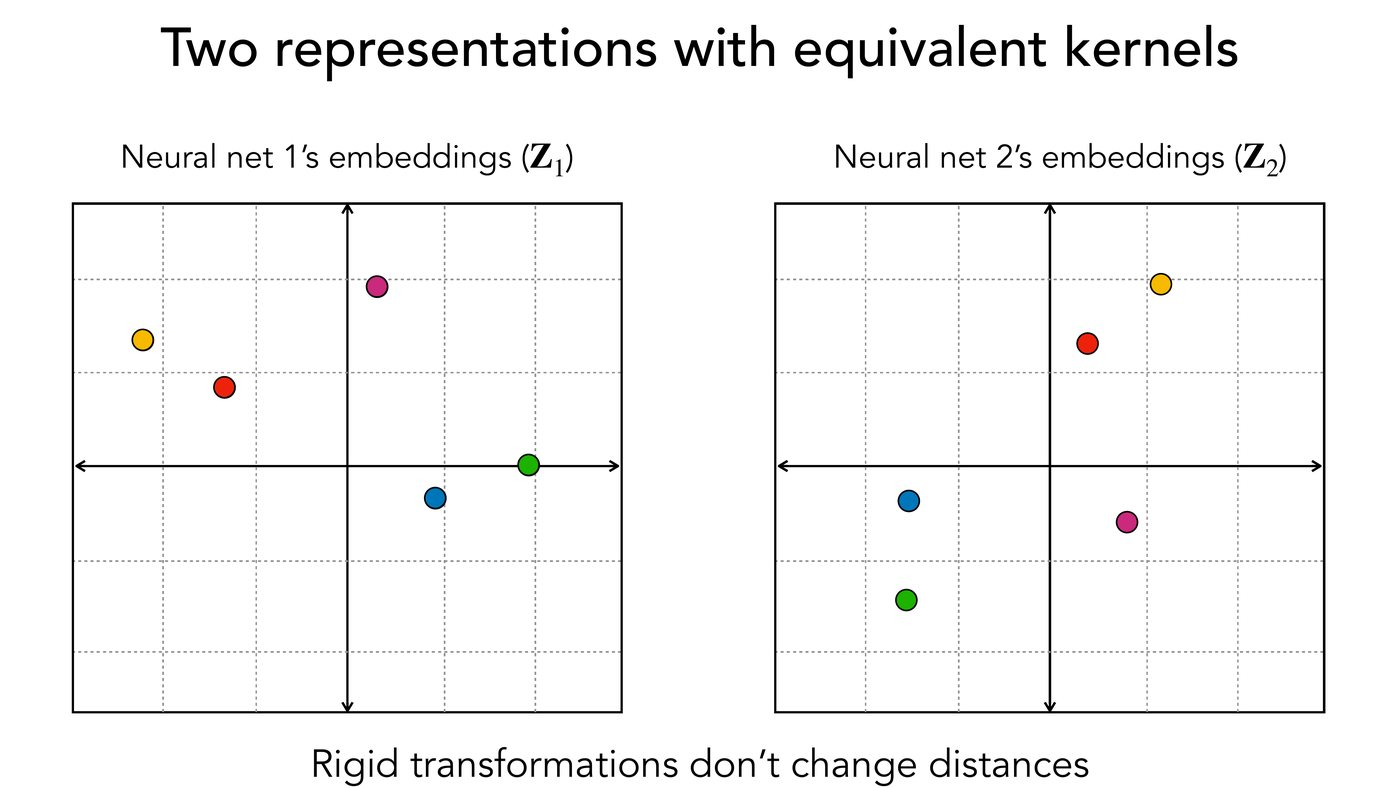
\includegraphics[width=0.82\textwidth]{figures/representational-geometry-1.jpg}
\caption{The invariance Isola argues for, from the Representational Geometry lecture. The
two panels hold the same five points related by a rigid transformation: every coordinate
changes, no pairwise distance does. The kernels are therefore identical and the two networks
count as the same representation, whereas a coordinate-wise comparison sees two unrelated
clouds.}
\label{fig:representational-geometry-1}
\end{figure}

\begin{figure}[htbp]
\centering
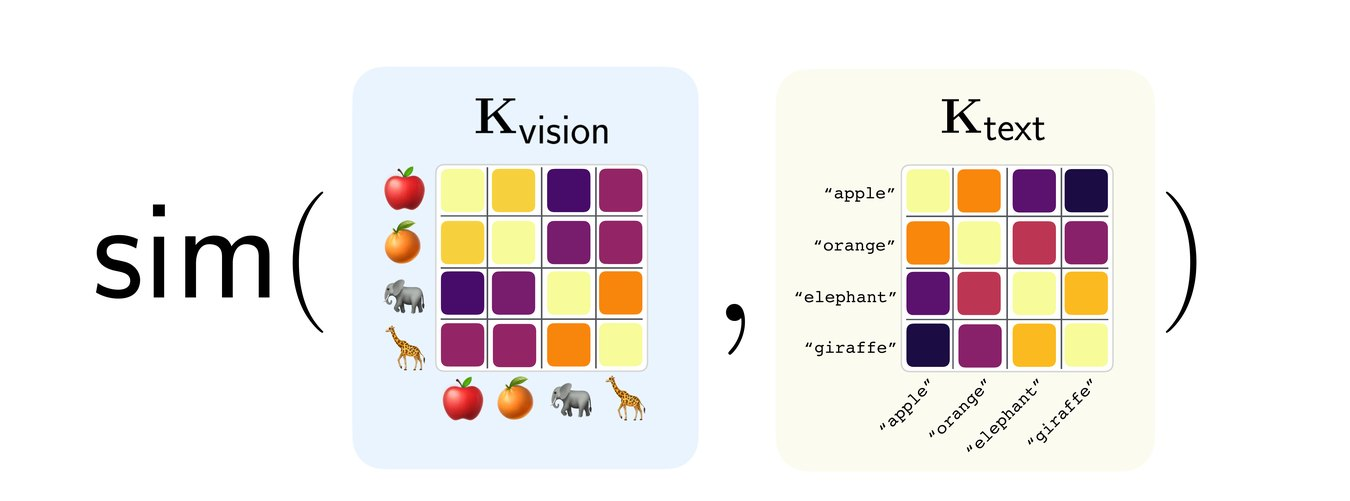
\includegraphics[width=0.86\textwidth]{figures/representational-geometry-2.jpg}
\caption{What cross-modal comparison actually compares, from the Representational Geometry
lecture. Each model is reduced to its own kernel matrix over the same four concepts, one from
images and one from the words naming them, and the two matrices are then compared. Nothing
requires the embeddings to share a dimension or a basis, only that both induce distances over
the same items.}
\label{fig:representational-geometry-2}
\end{figure}

\paragraph{Convergence, measured against humans and across modalities.} With a metric fixed,
the empirical section asks which representations actually agree. Against human similarity
judgements collected in DreamSim~\citep{fu2023}, DINO~\citep{caron2021} came out closest,
which is notable because DINO is trained on no human judgements at all. The same machinery,
borrowed from representational similarity analysis in neuroscience~\citep{kriegeskorte2008,
yamins2014}, then compares a vision model to a language model by asking whether their kernels
are alike (Figure~\ref{fig:representational-geometry-2}). The reported answer is that stronger
models converge, and that alignment increases with scale and over
time~\citep{huh2024}, which is the trend in
Figure~\ref{fig:representational-geometry-3}.\footnote{The personal notes add a caveat absent from the
slides, that open-source LLMs ``hasn't really increased though''. Recorded as a contemporaneous
observation, not as a lecture claim.} The lecture refuses to leave ``same'' vague and
offers three hypotheses: convergence to the same embedding vectors (identity), to the same
global kernel (glocal isometry), or to the same local neighbourhoods and clusters (local
ordinal isometry). Two theoretical results are sketched. A contrastive learner with an NCE
objective converges to pointwise mutual information,
\[
  \inner{\rep(\xin_a)}{\rep(\xin_b)} \;\approx\;
  \log \frac{P_{\text{co}}(\xin_a, \xin_b)}
            {P_{\text{co}}(\xin_a)\,P_{\text{co}}(\xin_b)},
\]
\noindent so for bijective discrete observation functions the PMI over observations equals
the PMI over underlying events, which forces different modalities onto the same kernel.
Separately, two CLIP-like models are claimed to converge to representations related by an
orthogonal transform $\mat{Q}$~\citep{gupta2026}.

\begin{figure}[htbp]
\centering
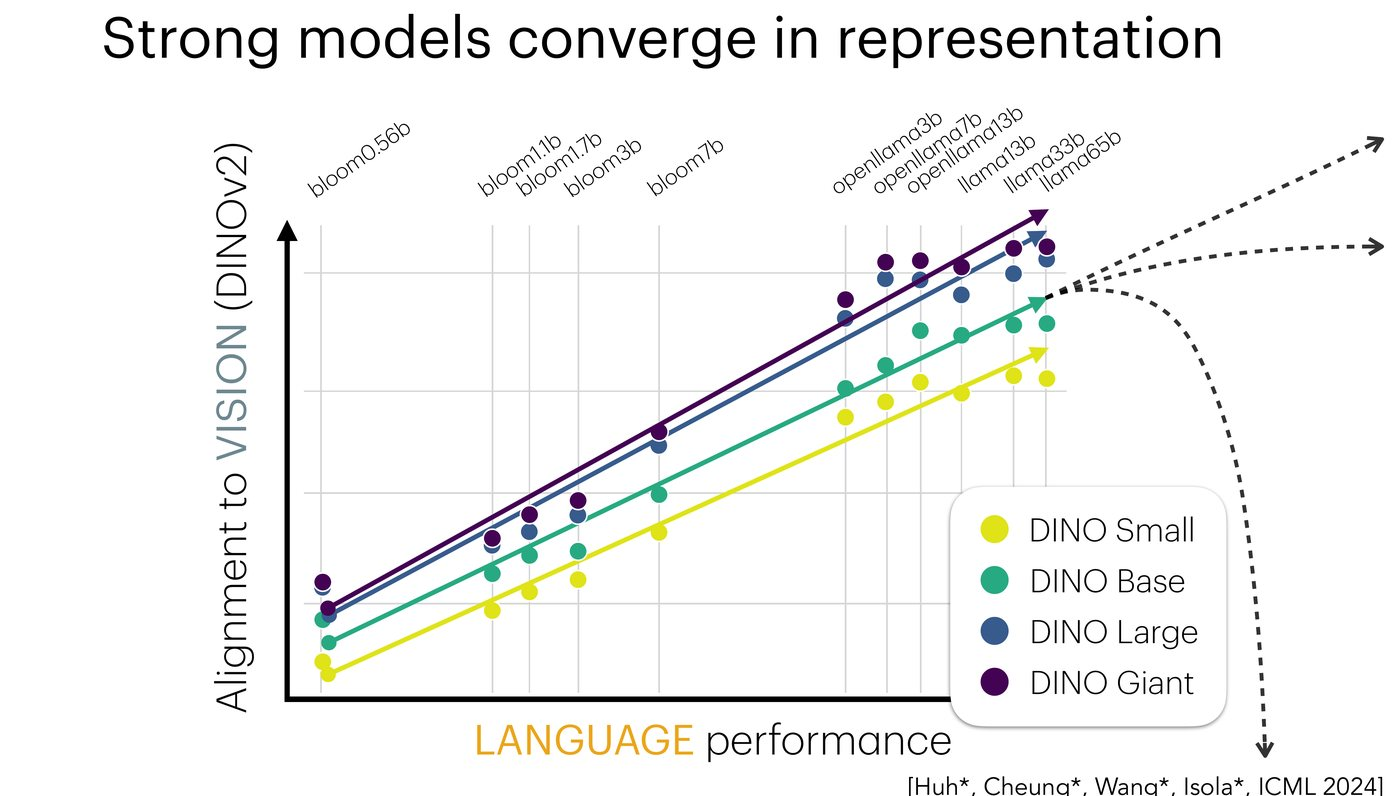
\includegraphics[width=0.84\textwidth]{figures/representational-geometry-3.jpg}
\caption{The central empirical claim of the Representational Geometry lecture. Alignment of a
language model's kernel to a vision model's (DINOv2) rises with the language model's own
performance, across the BLOOM and LLaMA families and across four DINO sizes. Better language
models look more like vision models, without ever having seen an image.}
\label{fig:representational-geometry-3}
\end{figure}

\paragraph{Alignment as a target, and what it costs.} If models converge anyway, alignment can
be engineered. Aligned representations let models share supervision and data, and a common
representation is a bridge for translation. The striking part is that paired data is not
required: vec2vec translates between embedding spaces using a GAN with a cycle-consistency
loss and a kernel-matching loss~\citep{jha2025}, an idea with a direct ancestor in
unsupervised word translation~\citep{conneau2018}, while REPA aligns a generative model's
representation to a pretrained one~\citep{yu2024}. Isola then lists the detriments without
softening them: alignment reduces diversity in the population of models; where one modality
has access to qualitatively different information, alignment destroys exactly that
information; and there may be no single best representation for all problems, which he notes
is not merely a practical worry but true in theory.

\section*{Notation}

$\rep$ and $\repB$ denote representations, $z = \rep(\xin)$ an embedding, $Z$ a point cloud
over a dataset, $h$ a map fitted between two embeddings, $\kernel$ a kernel matrix and $\Hcent$ the
centring matrix. One clash to
watch: $\Hcent$ here is a centring matrix, whereas
Chapter~\ref{ch:10-efficient-learning} uses $\Hess$ for a Hessian. Both follow their speaker's
usage and are kept visually distinct throughout.

\section*{Why it matters}

This is the lecture the personal notes cover in most detail, and it connects outward more than any
other. The claim that distance is the only thing worth preserving is the same
instinct that drives geometric deep learning
(Chapter~\ref{ch:11-geometric-deep-learning}), where invariance is imposed by construction
rather than measured after the fact. The convergence story is a counterpoint to Cho on
estimation (Chapter~\ref{ch:05-statistics-estimation}): Isola measures agreement between two
learned objects, Cho asks whether a learned estimator is even unbiased. And the tension
between alignment and diversity bears directly on CLIP's contrastive objective, which the summer
school's multimodal tutorial builds from scratch, since that loss is precisely the mechanism the
theory here predicts will drive convergence.

\begin{aside}
Isola's stronger claim, recorded in the personal notes rather than on the slides, is that
there is ``no future for distance functions that are not learned''. That sits in tension with
the argument of the lecture, which uses fixed metrics such as CKA to establish convergence.
If the yardstick is itself fitted to the objects being measured, the finding that models
converge becomes harder to state without circularity. Worth settling before leaning on
either claim.
\end{aside}
